\documentclass[a4paper,11pt]{article}

%-----------------------------------------

\usepackage[utf8]{inputenc} %Wegen Umlaute
\usepackage[ngerman]{babel} %Wegen Umlaute
\usepackage[T1]{fontenc} %pdf umlaute gefunden
\usepackage{graphicx}
%\usepackage{hyperref}
%\usepackage{floatflt,epsfig} 
\usepackage{float}%für bilder und grafiken
\usepackage{listings}
\lstset{language=VHDL, basicstyle=\small \ttfamily,  showtabs=false, keywordstyle=\bfseries, 
showstringspaces=false, framexleftmargin= 8mm, framexrightmargin= 15.4mm, frame=single, numbers=left, numberstyle=\tiny, stepnumber=1}
\usepackage{amsmath,bm}
\usepackage{chngcntr} %Abbildungsnummer 
\usepackage{caption}
\usepackage[absolute]{textpos}
\usepackage{courier}

%-----------------------------------------


\begin{document}


%\maketitle
\begin{titlepage}

\begin{textblock*}{70mm}(120mm,20mm)
    
\includegraphics[width=232px,height=46px]{HSFuldaLogo.pdf}
    \end{textblock*}

    \begin{center}
    \huge \textbf{\textsf{FD-Netzwerk}} \\
    \vspace{0.5cm}

\begin{figure}[H]
\centering
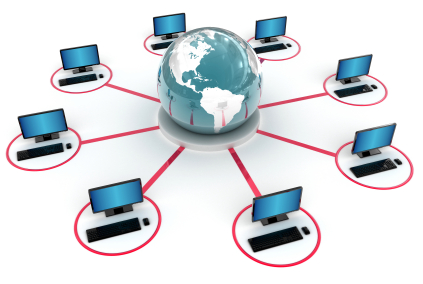
\includegraphics[width=0.4\textwidth]{network.jpg}
\numberwithin{figure}{section}
%\caption{Netzwerk}
\end{figure}
$~~$\\


    \normalsize
    vorgelegt am: \today \\
    \vspace{0.5cm}
    \large \textbf{Fachbereich~Angewandte Informatik \\Hochschule~Fulda}\\
    \vspace{0.5cm}
    \huge \textbf{Planung und Durchführung vom Netzwerkprojekt}\\
    \vspace{0.5cm}
    \large \textbf{Prof. Dr.-Ing Anatol Badach}\\
    \vspace{0.5cm}
    \large{SS16}
    \vspace{0.5cm}
    \end{center}
 \normalsize{
    \begin{tabular}{ll}
    	Name: & {Hakan Cihan} \\
    	%Matrikelnummer: & {431746} \\
    	Email: & {hakan.cihan@informatik.hs-fulda.de} \\
    	\\
    	Name: & {Kevin Klüber} \\
    	%Matrikelnummer: & {134880} \\
    	Email: & {kevin.klueber@informatik.hs-fulda.de} \\
    	\\
    	Name: & {Marvin Klüber} \\
    	%Matrikelnummer: & {132243} \\
    	Email: & {marvin.klueber@informatik.hs-fulda.de} \\
	\\
    	Name: & {Jakob Stockmayer} \\
    	%Matrikelnummer: & {239792} \\
    	Email: & {jakob.stockmayer@informatik.hs-fulda.de} \\
	\\
    	Name: & {Lukas Wegstein} \\
    	%Matrikelnummer: & {139018} \\
    	Email: & {lukas.wegstein@informatik.hs-fulda.de} \\
	 \\
    	
    \end{tabular}\\
    }
\end{titlepage}
\newpage
\tableofcontents
\newpage
\makeatletter
\renewcommand{\l@figure}{\@dottedtocline{1}{0cm}{1.2cm}}
\makeatother
\listoffigures
\newpage

\section{IST-Analyse}
Unsere Aufgabe ist ein Netzwerk für eine Firma zu realisieren. Die Firma besitzt vier Gebäude und ca. 500 Angestellte. Es gibt drei kleinere Gebäude die drei Etagen besitzen und ein großes Gebäude mit 4 Etagen und einem Keller, wo sich das Datacenter befindet. In den kleineren Gebäuden sind jeweils 100 angestellte und in dem Großen 200. Alle Gebäude befinden sich noch im Rohbau. 
\\
\subsection{Mögliche Schwachstellen}
    \begin{itemize}
        \item große Broadcast-Domain
        \item nicht aktuelle Netzwerkdokumentation
        \\
    \end{itemize}

\subsection{Zielvorstellungen}
    \begin{itemize}
        \item Skalierbarkeit
        \item Ausfallsicherheit
        \\
    \end{itemize}




\section{SOLL-Analyse}
\subsection{Projektanforderungen}
Von der Geschäftsleitung wurde eine Anzahl an Anforderungen gestellt. Diese sollen hier kurz erläutert werden:
\subsubsection{Skalierbarkeit und Zukunftssicherheit}
Die Firma soll auch in Zukunft wachsen. Sowohl die neuen Gebäude als auch die dazugehörige Infrastruktur soll diesem geplanten Wachstum Rechnung tragen. Da durch den Umzug die Chance zur kompletten Neuinstallation der Netzwerktechnik besteht, sollte diese bei dieser Gelegenheit zukunftssicher ausgelegt sein.

\subsubsection{Ausfallsicherheit}
In den alten Geschäftsräumen kam es immer wieder zu Netzwerkausfällen durch defekte Hardware. Dies führte zu hohen Ausfallzeiten und daher zu Beeinträchtigungen der gesamten Firma, welche unnötige finanzielle Schäden nach sich zogen. Um dies zu verhindern soll das neue Netzwerk mit dem Ziel entwickelt werden, hohe Ausfallsicherheit zu gewährleisten.

\subsubsection{Performance}
Über das Netzwerk werden große Datenmengen übertragen. Lange Übertragungszeiten führen zu unnötigen Wartezeiten bei den Nutzern. Dies verschwendet einerseits zu Arbeitszeit, andererseits reduzieren langsame Systeme die Arbeitsqualität deutlich.

\subsubsection{Schnelle Internetanbindung}
Das Unternehmen steht regelmäßig im Austausch mit anderen Firmen. Bei Partnerschaften werden regelmäßig Daten im Netzwerk der Firma gehostet. Diese dürfen die Firma aufgrund von Sicherheitsvorschriften nicht verlassen und werden daher zu den Unternehmspartnern gestreamt. Hierfür ist eine potente Internetleitung nötig, da sowohl Upload als auch Download stark belastet werden können.

\subsection{Projektrandbedingungen}
Durch den Umzug in neue Gebäudekomplexe ist die Verkabelung komplett neu zu realisieren. Daher ergeben sich aus dieser Sicht keine Einschränkungen.
Weiterhin ist der Geschäftsleitung ein performantes und ausfallsicheres System sehr wichtig. Daher stellt diese ein ausreichend großes Budget zur Verfügung. Zur Kostenreduzierung sollen alte, schnell ersetzbare und ausfallsichere Komponenten wie Layer2- Switches wiederverwendet werden.
\\
Die neuen Firmengebäude befinden sich in der Nähe eines Internetknotenpunktes. Es sind Leerrohre zwischen den einzelnen Gebäuden verlegt. Jedes Gebäude verfügt über eine separate Stromversorgung.

\subsection{Risiken}
Durch die hohe Anzahl der Mitarbeiter können große Kollisionsdomänen entstehen. Diese führen unter Umständen zu sogenannten „Broadcast-Storms“, welche große Teile der Netzwerkleitung belegen.
\\
Ein Ausfall zentraler Komponenten könnte zum Ausfall der gesamten Firma führen. Es ist eine wesentliche Anforderung der Geschäftsleitung dies zu verhindern.
Durch einen Stromausfall im Rechenzentrum der Firma können wichtige Daten verloren gehen oder korrumpiert werden.

\subsection{Umsetzungsmöglichkeiten}
Die ambitionierten Projektanforderungen werden nicht durch ein enges Budget begrenzt. Es wurde daher die im logischen Netzwerkplan zu sehende Topologie entworfen. Diese erfüllt die Anforderungen wie folgt:
\\
\\
Kritische Komponenten werden redundant ausgelegt (AS, CS). Von diesen darf eine ausfallen, ohne die Funktion des Netzwerkes zu kompromittieren. Sie sind so ausgelegt, dass die verbliebene Komponente die Mehrleistung auffangen kann. 
\\
\\
Das Datenzentrum ist mit USPs ausgestattet. Diese sind groß genug ausgelegt, als das im Falle eines Stromausfalls ein Herunterfahren der Server in 10 Minuten gesichert werden kann. Dies gibt genug Zeit um kritische Daten zu sichern, sodass keine Datenverluste drohen.
\\
\\
Gegen einen Stromausfall in den restlichen Gebäuden werden keine Maßnahmen getroffen, da hier eine Lösung nicht wirtschaftlich wäre.
Es sind zwei Internetleitungen vorhanden. Durch den Sitz Nähe eines Internetknotenpunktes  und dem Neubau der Gebäude kann eine der beiden Leitungen per Glasfaser direkt bis in die Zentrale gelegt werden. Diese Leitung garantiert die hohen Übertragungsraten, die für die Belegschaft und das Datenstreaming zu Kunden benötigt wird. Als Backupleitung wird eine synchrone 100Mbit/s-Leitung verwendet. Mit den ISPs werden entsprechende SL-Agreements zur Verfügbarkeit abgeschlossen.
\\
\\
Im Core-Bereich und im Rechenzentrum werden Glasfaserkabel verwendet. Diese garantieren auf lange Zeit die Zukunftssicherheit des Systems durch sehr hohe Übertragungsraten.
\\
\\
Für die Gebäude A, B und C wird jeweils ein eigenes Subnetz gebildet. Dieses wird an der Stelle der DS verwaltet. In den Gebäuden werden in jedem Stockwerk zwei Layer-2-Switche verwendet. Diese sind alte 40-Port Switche, Sie werden aus dem vorherigen Firmengebäude übernommen. Jeder der ist mit beiden DS eines Gebäudes verbunden. Ein Ausfall eines DS kann so kompensiert werden. Beim Ausfall eines der Layer-2-Switche müssen die Kabel des jeweiligen L2S auf den anderen L2S umgesteckt werden. Diese bieten genug Steckplätze, um problemlos einen Ausfall zu kompensieren. Durch die erhöhte Anzahl an Steckplätzen sind diese auch Zukunftssicher.
Zwischen DS und den L2-Switchen werden Cat-7-Ethernetkabel verwendet, von den L2S zu den Endbenutzerplätzen wird Cat 6 eingesetzt.
\\
\\
In der Zentrale wird ein Subnetz pro Etage gebildet. Dies verkleinert die Kollisionsdomänen wesentlich. Weiterhin erleichtert es das spätere Wachstum, da mehr Adressen pro Subnetz zur Verfügung stehen. Die Switche auf der Etagenebene werden mit 100 Steckplätzen ausgelegt und arbeiten auf Layer 3.














\end{document}